% Created 2013-01-23 Wed 22:17
\documentclass[table]{beamer}
\usepackage[utf8]{inputenc}
\usepackage[T1]{fontenc}
\usepackage{fixltx2e}
\usepackage{graphicx}
\usepackage{longtable}
\usepackage{float}
\usepackage{wrapfig}
\usepackage{soul}
\usepackage{textcomp}
\usepackage{marvosym}
\usepackage{wasysym}
\usepackage{latexsym}
\usepackage{amssymb}
\usepackage{hyperref}
\tolerance=1000
\usepackage{tikz}
\usepackage{minted}
\usepackage{fancyvrb}
\usemintedstyle{perldoc}
\definecolor{lightgray}{gray}{0.9}
\setlength{\tabcolsep}{1ex}
\institute{IQSS}
\usetheme{Warsaw}
\useoutertheme{infolines}
\titlegraphic{
\includegraphics[width=.75\textwidth]{images/IQSSNewLogo.pdf}}
\AtBeginSection[]{\begin{frame}<beamer>\frametitle{Topic}\tableofcontents[currentsection]\end{frame}}
\providecommand{\alert}[1]{\textbf{#1}}

\title{Data Management in Stata}
\author{Ista Zahn}
\date{January 24 2013}
\hypersetup{
  pdfkeywords={},
  pdfsubject={},
  pdfcreator={Emacs Org-mode version 7.9.3d}}

\begin{document}

\maketitle

\begin{frame}
\frametitle{Outline}
\setcounter{tocdepth}{3}
\tableofcontents
\end{frame}







\section{Introduction}
\label{sec-1}

\rowcolors{1}{blue!15}{blue!3}
\definecolor{bg}{rgb}{0.95,0.95,0.95}
\definecolor{cbg}{cmyk}{0,0,.1,0}
\begin{frame}[fragile]
\frametitle{Copy the workshop materials to your home directory}
\label{sec-1-1}


\begin{itemize}
\item \textbf{Log in to an Athena workstation} using your Athena user name and password
\item \textbf{Click on the ``Ubuntu'' button} on the upper-left and type ``term'' as shown below
\end{itemize}
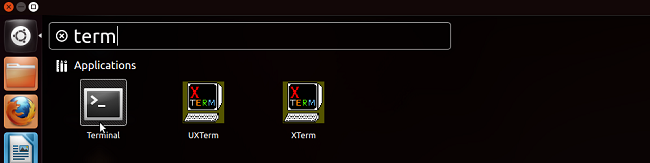
\includegraphics[width=.8\textwidth]{./images/OpenTerminal.png}

\begin{itemize}
\item \textbf{Click on the ``Terminal'' icon} as shown above
\item In the terminal, \textbf{type this line exactly as shown}:
\end{itemize}
{\footnotesize
\begin{verbatim}
 cd; wget http://tinyurl.com/statadatman-zip; unzip statadatman-zip
\end{verbatim}
\normalsize}

\begin{itemize}
\item If you see ``ERROR 404: Not Found'', then you mistyped the command -- try again, making sure to type the command exactly as shown
\end{itemize}
\end{frame}
\begin{frame}[fragile]
\frametitle{Launch Stata on Athena}
\label{sec-1-2}


\begin{itemize}
\item To start Stata \textbf{type these commands in the terminal}:
\end{itemize}
\begin{verbatim}
     add stata
     xstata
\end{verbatim}
\begin{itemize}
\item Open up today's Stata script
\begin{itemize}
\item In Stata, go to \textbf{Window => New do file => Open}
\item Locate and open the \texttt{StatDatMan.do} script in the StataDatMan folder in your home directory
\end{itemize}
\item I encourage you to add your own notes to this file!
\end{itemize}
\end{frame}
\begin{frame}
\frametitle{Workshop Description}
\label{sec-1-3}

\begin{itemize}
\item This is an Introduction to data management in Stata
\item Assumes basic knowledge of Stata
\item Not appropriate for people already well familiar with Stata
\item If you are catching on before the rest of the class, experiment with command features described in help files
\end{itemize}
\end{frame}
\begin{frame}
\frametitle{Organization}
\label{sec-1-4}

\begin{itemize}
\item Please feel free to ask questions at any point if they are relevant to the current topic (or if you are lost!)
\item There will be a Q\&A after class for more specific, personalized questions
\item Collaboration with your neighbors is encouraged
\item If you are using a laptop, you will need to adjust paths accordingly
\end{itemize}
\end{frame}
\begin{frame}[fragile]
\frametitle{Opening Files in Stata}
\label{sec-1-5}

\begin{itemize}
\item Look at bottom left hand corner of Stata screen
\begin{itemize}
\item This is the directory Stata is currently reading from
\end{itemize}
\item Files are located in the StataDatMan folder on the Desktop
\item Start by telling Stata where to look for these
\end{itemize}
\vspace{-.5em} \begin{columns} \column{.85\linewidth} \begin{block}{}

\begin{minted}[fontsize=\footnotesize]{c}
// change directory
cd "C:/Users/dataclass/Desktop/StataDatMan"

// Use dir to see what is in the directory:
dir

// use the gss data set
use gss.dta
\end{minted}
\end{block} \end{columns}
\end{frame}
\section{Generating and replacing variables}
\label{sec-2}
\begin{frame}
\frametitle{Logic Statements Useful Data Manipulation}
\label{sec-2-1}


\begin{description}
\item[==] equal to (status quo)
\item[=] used in assigning values
\item[!=] not equal to
\item[>] greater than
\item[>=] greater than or equal to
\item[\&] and
\item[|] or
\end{description}
     
\end{frame}
\begin{frame}
\frametitle{Basic Data Manipulation Commands}
\label{sec-2-2}

\begin{itemize}
\item Basic commands you'll use for generating new variables or recoding existing variables:
\begin{itemize}
\item egen
\item replace
\item recode
\end{itemize}
\item Many different means of accomplishing the same thing in Stata
\begin{itemize}
\item Find what is comfortable (and easy) for you
\end{itemize}
\end{itemize}
\end{frame}
\begin{frame}[fragile]
\frametitle{Generate and Replace}
\label{sec-2-3}

\begin{itemize}
\item The \verb~gen~ command is often used with logic statements, as in this example:
\end{itemize}
\vspace{-.5em} \begin{columns} \column{.85\linewidth} \begin{block}{}

\begin{minted}[fontsize=\footnotesize]{c}
// create "hapnew" variable
gen hapnew = . //set to missing
//set to 1 if happy equals 1
replace hapnew=1 if happy==1 
//set to 1 if happy and hapmar = 3
replace hapnew=1 if happy>3 & hapmar>3
//set to 3 if happy or hapmar = 4
replace hapnew=3 if happy>4 | hapmar>4
tab hapnew // tabulate the new variable
\end{minted}
\end{block} \end{columns}
\end{frame}
\begin{frame}[fragile]
\frametitle{Recode}
\label{sec-2-4}

\begin{itemize}
\item The \verb~recode~ command is basically generate and replace combined
\item You can recode an existing variable OR use recode to create a new variable
\end{itemize}

\vspace{-.5em} \begin{columns} \column{.85\linewidth} \begin{block}{}

\begin{minted}[fontsize=\footnotesize]{c}
// recode the wrkstat variable 
recode wrkstat (1=8) (2=7) (3=6) (4=5) (5=4) (6=3) (7=2) (8=1)
// recode wrkstat into a new variable named wrkstat2
recode wrkstat (1=8), gen(wrkstat2)
// tabulate workstat
tab wrkstat
\end{minted}
\end{block} \end{columns}
\end{frame}
\begin{frame}
\frametitle{Basic Rules for Recode}
\label{sec-2-5}


\begin{center}
\begin{tabular}{lll}
 Rule           &  Example    &  Meaning                   \\
\hline
 \#=\#          &  3=1        &  3 recoded to 1            \\
 \#\#=\#        &  2. =9      &  2 and . recoded to 9      \\
 \#/\# = \#     &  1/5=4      &  1 through 5 recoded to 4  \\
 nonmissing=\#  &  nonmiss=8  &  nonmissing recoded to 8   \\
 missing=\#     &  miss=9     &  missing recoded to 9      \\
\end{tabular}
\end{center}
\end{frame}
\begin{frame}[fragile]
\frametitle{egen}
\label{sec-2-6}

\begin{itemize}
\item \verb~egen~ means ``extension'' to generate
\item Contains a variety of more sophisticated functions
\item Type ``help egen'' in Stata to get a complete list of functions
\item Let's create a new variable that counts the number of ``yes'' responses on computer, email and internet use:
\end{itemize}
\vspace{-.5em} \begin{columns} \column{.85\linewidth} \begin{block}{}

\begin{minted}[fontsize=\footnotesize]{c}
// count number of yes on comp email and interwebs 
egen compuser= anycount(usecomp usemail usenet), values(1)
tab compuser
// assess how much missing data each participant has:
egen countmiss = rowmiss(age-wifeft)
codebook countmiss
// compare values on multiple variables
egen ftdiff=diff(wkft//)
codebook ftdiff
\end{minted}
\end{block} \end{columns}
\end{frame}
\section{By processing}
\label{sec-3}
\begin{frame}[fragile]
\frametitle{The ``By'' Command}
\label{sec-3-1}

\begin{itemize}
\item Sometimes, you'd like to create variables based on different categories of a single variable
\begin{itemize}
\item For example, say you want to look at happiness based on whether an individual is male or female
\end{itemize}
\item The ``by'' prefix does just this:
\end{itemize}
\vspace{-.5em} \begin{columns} \column{.85\linewidth} \begin{block}{}

\begin{minted}[fontsize=\footnotesize]{c}
// tabulate happy separately for male and female 
bysort sex: tab happy
// generate summary statistics using bysort 
bysort state: egen stateincome = mean(income)
bysort degree: egen degreeincome = mean(income)
bysort marital: egen marincomesd = sd(income)
\end{minted}
\end{block} \end{columns}
\end{frame}
\begin{frame}[fragile]
\frametitle{The ``By'' Command}
\label{sec-3-2}

\begin{itemize}
\item Some commands won't work with by prefix, but have by options:
\end{itemize}
\vspace{-.5em} \begin{columns} \column{.85\linewidth} \begin{block}{}

\begin{minted}[fontsize=\footnotesize]{c}
// generate separate histograms for female and male 
hist happy, by(sex)
\end{minted}
\end{block} \end{columns}

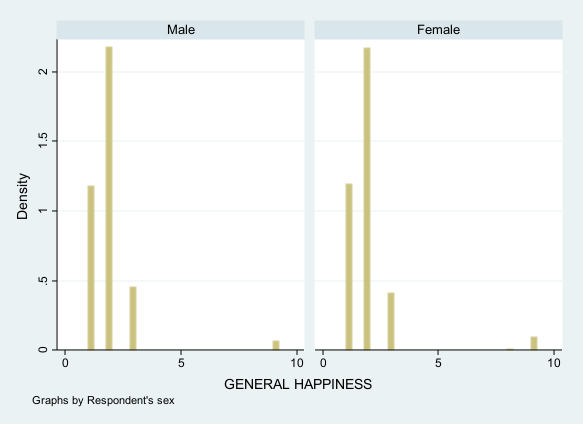
\includegraphics[width=.6\textwidth]{images/histBysex.png}
\end{frame}
\section{Missing values}
\label{sec-4}
\begin{frame}
\frametitle{Missing Values}
\label{sec-4-1}

\begin{itemize}
\item Always need to consider how missing values
  are coded when recoding variables
\item Stata's symbol for a missing value is ``.''
\item Stata interprets ``.'' as a large value
\begin{itemize}
\item What are implications of this?
\end{itemize}
\end{itemize}
\end{frame}
\begin{frame}[fragile]
\frametitle{Missing Values}
\label{sec-4-2}

\begin{itemize}
\item If we want to generate a new variable that identifies highly educated women, we might use the command:
\end{itemize}
\vspace{-.5em} \begin{columns} \column{.85\linewidth} \begin{block}{}

\begin{minted}[fontsize=\footnotesize]{c}
// generate and replace without considering missing values
gen hi_ed=0
replace hi_ed=1 if wifeduc>15
// What happens to our missing values when we
tab hi_ed, mi nola
// Instead, we might try:
drop hi_ed
// gen hi_ed, but don't set a value if wifeduc is missing
gen hi_ed = 0 if wifeduc != . 
// only replace non-missing
replace hi_ed=1 if wifeduc >15 & wifeduc !=. 
tab hi_ed, mi //check to see that missingness is preserved
\end{minted}
\end{block} \end{columns}

\begin{itemize}
\item Note that you need the ``mi'' option to tab to view your
  missing data values
\end{itemize}
\end{frame}
\begin{frame}[fragile]
\frametitle{Missing Values}
\label{sec-4-3}

\begin{itemize}
\item What if you used a numeric value originally to code
  missing data (e.g., ``999'')?
\item The mvdecode command will convert all these values to
  missing
\end{itemize}
\vspace{-.5em} \begin{columns} \column{.85\linewidth} \begin{block}{}

\begin{minted}[fontsize=\footnotesize]{c}
mvdecode _all, mv(999)
\end{minted}
\end{block} \end{columns}

\begin{itemize}
\item The ``\_all'' command tells Stata to do this to all variables
\item Use this command carefully!
\begin{itemize}
\item If you have any variables where ``999'' is a legitimate value,
     Stata is going to recode it to missing
\item As an alternative, you could list var names separately rather
     than using ``\_all'' command
\end{itemize}
\end{itemize}
\end{frame}
\section{Variable types}
\label{sec-5}
\begin{frame}
\frametitle{Variable Types}
\label{sec-5-1}

\begin{itemize}
\item Stata uses two main types of variables: String
  and Numeric
\item String variables are typically used for text
  variables
\item To be able to perform any mathematical
  operations, your variables need to be in a
  numeric format
\end{itemize}
\end{frame}
\begin{frame}[fragile]
\frametitle{Variable Types}
\label{sec-5-2}

\begin{itemize}
\item Stata's numeric variable types:
\end{itemize}


\vspace{-.5em}
 \begin{columns}
 \column{.95\linewidth}
 \begin{block}{}
 \begin{minted}[linenos=true, fontsize=\footnotesize]{c}
type                 Minimum              Maximum    being 0     bytes
----------------------------------------------------------------------
byte                    -127                  100    +/-1          1
int                  -32,767               32,740    +/-1          2
long          -2,147,483,647        2,147,483,620    +/-1          4
float   -1.70141173319*10^38 1.70141173319*10^38     +/-10^-38     4
double -8.9884656743*10^307 8.9884656743*10^307      +/-10^-323    8
----------------------------------------------------------------------
Precision for float is 3.795x10^-8.
Precision for double is 1.414x10^-16.
\end{minted}
 \end{block}
 \end{columns}
 \vspace{.25em}
 
\end{frame}
\begin{frame}[fragile]
\frametitle{Variable Types}
\label{sec-5-3}

\begin{itemize}
\item How can I deal with those annoying string
  variables?
\item Sometimes you need to convert to/from string variables
\end{itemize}
\vspace{-.5em} \begin{columns} \column{.85\linewidth} \begin{block}{}

\begin{minted}[fontsize=\footnotesize]{c}
// not run; generate "newvar" equal to numeric version of var2
destring var1, gen(newvar)
// not run; convert var1 to string.
tostring var1, gen(newvar)
\end{minted}
\end{block} \end{columns}
\end{frame}
\begin{frame}
\frametitle{Date and Time Variable Types}
\label{sec-5-4}

\begin{itemize}
\item Stata offers several options for date and time
  variables
\item Generally, Stata will read date/time variables as
  strings
\item You'll need to convert string variables in order to
  perform any mathematical operations
\item Once data is in date/time form, Stata uses
  several symbols to identify these variables
\begin{itemize}
\item \%tc, \%td, \%tw, etc.
\end{itemize}
\end{itemize}
\end{frame}
\begin{frame}[fragile]
\frametitle{Variable Types: Date and Time}
\label{sec-5-5}



\vspace{-.5em}
 \begin{columns}
 \column{.95\linewidth}
 \begin{block}{}
 \begin{minted}[linenos=true, fontsize=\footnotesize]{c}
Format String-to-numeric conversion function
    -------+-----------------------------------------
    %tc     clock(string, mask)
    %tC     Clock(string, mask)
    %td     date(string, mask)
    %tw     weekly(string, mask)
    %tm     monthly(string, mask)
    %tq     quarterly(string, mask)
    %th     halfyearly(string, mask)
    %ty     yearly(string, mask)
    %tg     no function necessary; read as numeric
    -------------------------------------------------
\end{minted}
 \end{block}
 \end{columns}
 \vspace{.25em}
 
\end{frame}
\begin{frame}
\frametitle{Variable Types: Date and Time}
\label{sec-5-6}



\begin{center}
\begin{tabular}{lllll}
 Format  &  Meaning     &  Value = -1    &  Value = 0     &  Value = 1     \\
\hline
 \%tc    &  clock       &  31dec1959     &  01jan1960     &  01jan1960     \\
         &              &  23:59:59.999  &  00:00:00.000  &  00:00:00.001  \\
 \%td    &  days        &  31dec1959     &  01jan1960     &  02jan1960     \\
 \%tw    &  weeks       &  1959w52       &  1960w1        &  1960w2        \\
 \%tm    &  months      &  1959m12       &  1960m1        &  1960m2        \\
 \%tq    &  quarters    &  1959q4        &  1960q1        &  1960q2        \\
 \%th    &  half-years  &  1959h2        &  1960h1        &  1960h2        \\
 \%tg    &  generic     &  -1            &  0             &  1             \\
\end{tabular}
\end{center}
\end{frame}
\begin{frame}[fragile]
\frametitle{Variable Types: Date and Time}
\label{sec-5-7}

\begin{itemize}
\item To convert a string variable into date/time
  format, first select the date/time format you'll
  be using (e.g., \%tc, \%td, \%tw, etc.)
\item Let's say we create a string variable, today's
  date (today) that we want to format
\end{itemize}

\vspace{-.5em} \begin{columns} \column{.85\linewidth} \begin{block}{}


\begin{minted}[fontsize=\footnotesize]{c}
// create string variable and convert to date
gen today = "Feb 18, 2011"
gen date1 = date(today, "MDY")
tab date1
// use the format command to change how the date is displayed
// format so humans can read the date
format date1 %d
tab date1
\end{minted}
\end{block} \end{columns}
\end{frame}
\begin{frame}[fragile]
\frametitle{Variable Types}
\label{sec-5-8}

\begin{itemize}
\item What if you have a variable ``time'' formatted as DDMMYYYYhhmmss?
\end{itemize}
\vspace{-.5em} \begin{columns} \column{.85\linewidth} \begin{block}{}

\begin{minted}[fontsize=\footnotesize]{c}
// Not run: conceptual example only
generate double time2 = clock(time, "DMYHMS")
tab time2
format time2 %tc
tab time2
\end{minted}
\end{block} \end{columns}

\begin{itemize}
\item ``double'' command necessary for all clock formats
\item basically tells Stata to allow a long string of
     characters
\end{itemize}
\end{frame}
\begin{frame}
\frametitle{Exercise 1: Generate, Replace, Recode \& Egen}
\label{sec-5-9}

Open the datafile, gss.dta.
\begin{enumerate}
\item Generate a new variable that represents the squared value of age.
\item Recode values ``99'' and ``98'' on the variable, ``hrs1''  as ``missing.''
\item Generate a new variable equal to ``1'' if income is greater than ``19''.
\item Recode the marital variable into a ``string'' variable and then back into a numeric variable.
\item Create a new variable that counts the number of times a respondent answered ``don't know'' in regard to the following variables: life, richwork, hapmar.
\item Create a new variable that counts the number of missing responses for each respondent.
\item Create a new variable that associates each individual with the average number of hours worked among individuals with matching educational degrees.
\end{enumerate}
\end{frame}
\section{Merging, appending, and joining}
\label{sec-6}
\begin{frame}
\frametitle{Merging Datasets}
\label{sec-6-1}

\begin{itemize}
\item Merge in Stata is for adding new variables
  from a second dataset to the dataset you're
  currently working with
\begin{itemize}
\item Current active dataset = master dataset
\item Dataset you'd like to merge with master = using
     dataset
\end{itemize}
\item If you want to add OBSERVATIONS, you'd use
  ``append'' (we'll go over that next)
\end{itemize}
\end{frame}
\begin{frame}
\frametitle{Merging Datasets}
\label{sec-6-2}

\begin{itemize}
\item Several different ways that you might be
  interested in merging data
\begin{itemize}
\item Two datasets with same participant pool, one row
     per participant (1:1)
\item A dataset with one participant per row with a
     dataset with multiple rows per participant
     (1:many or many:1)
\end{itemize}
\end{itemize}
\end{frame}
\begin{frame}[fragile]
\frametitle{Merging Datasets}
\label{sec-6-3}

\begin{itemize}
\item Stata will create a new variable (``\_merge'')
  that describes the source of the data
\begin{itemize}
\item Use option, ``nogenerate'' if you don't want
     \_merge created
\item Use option, ``generate(varname)'' to give $_{\mathrm{merge}}$
     your own variable name
\end{itemize}
\item Need to add IDs to your dataset?
\end{itemize}

\vspace{-.5em} \begin{columns} \column{.85\linewidth} \begin{block}{}

\begin{minted}[fontsize=\footnotesize]{c}
// create a variable "id" equal to the row number 
generate id = _n
\end{minted}
\end{block} \end{columns}
\end{frame}
\begin{frame}
\frametitle{Merging Datasets}
\label{sec-6-4}

\begin{itemize}
\item Before you begin:
\begin{itemize}
\item Identify the ``ID'' that you will use to merge your two datasets
\item Determine which variables you'd like to merge
\item In Stata >= 11, data does NOT have to be sorted
\item Variable types must match across datasets
\item Can use ``force'' option to get around this, but not recommended
\end{itemize}
\end{itemize}
\end{frame}
\begin{frame}[fragile]
\frametitle{Merging Datasets}
\label{sec-6-5}

\begin{itemize}
\item Let's say I want to perform a 1:1 merge using
  the dataset ``data2'' and the ID, ``participant''
\end{itemize}
merge 1:1 participant using data2.dta
\begin{itemize}
\item Now, let's say that I have one dataset with
  individual students (master) and another
  dataset with information about the students'
  schools called ``school''
\end{itemize}

\vspace{-.5em} \begin{columns} \column{.85\linewidth} \begin{block}{}

\begin{minted}[fontsize=\footnotesize]{c}
// Not run: conceptual example only. Merge school and student data
merge m:1 schoolID using school.dta
\end{minted}
\end{block} \end{columns}
\end{frame}
\begin{frame}[fragile]
\frametitle{Merging Datasets}
\label{sec-6-6}

\begin{itemize}
\item What if my school dataset was the master and
  my student dataset was the merging dataset?
\end{itemize}

\vspace{-.5em} \begin{columns} \column{.85\linewidth} \begin{block}{}

\begin{minted}[fontsize=\footnotesize]{c}
// Not run: conceptual example only.
merge 1:m schoolID using student.dta
\end{minted}
\end{block} \end{columns}
\begin{itemize}
\item It is also possible to do a many:many merge
\begin{itemize}
\item Data needs to be sorted in both the master and using datasets
\end{itemize}
\end{itemize}
\end{frame}
\begin{frame}
\frametitle{Merging Datasets}
\label{sec-6-7}

\begin{itemize}
\item Update and replace options:
\begin{itemize}
\item In standard merge, the master dataset is the
      authority and WON'T CHANGE
\item What if your master dataset has missing data and
     some of those values are not missing in your using
     dataset?
\item Specify ``update''- it will fill in missing without
     changing nonmissing
\end{itemize}
\item What if you want data from your using dataset to
    overwrite that in your master?
\begin{itemize}
\item Specify ``replace update''- it will replace master data
     with using data UNLESS the value is missing in the using
     dataset
\end{itemize}
\end{itemize}
\end{frame}
\begin{frame}[fragile]
\frametitle{Appending Datasets}
\label{sec-6-8}

\begin{itemize}
\item Sometimes, you'll have observations in two
  different datasets, or you'd like to add
  observations to an existing dataset
\item Append will simply add observations to the
  end of the observations in the master
\end{itemize}
\vspace{-.5em} \begin{columns} \column{.85\linewidth} \begin{block}{}

\begin{minted}[fontsize=\footnotesize]{c}
// Not run: conceptual example. add rows of data from dataset2 
append using dataset2
\end{minted}
\end{block} \end{columns}
\end{frame}
\begin{frame}[fragile]
\frametitle{Appending Datasets}
\label{sec-6-9}

\begin{itemize}
\item Some options with Append:
\begin{itemize}
\item generate(newvar) will create variable that
     identifies source of observation
\end{itemize}
\end{itemize}
\vspace{-.5em} \begin{columns} \column{.85\linewidth} \begin{block}{}

\begin{minted}[fontsize=\footnotesize]{c}
// Not run: conceptual example.
append using dataset1, generate(observesource)
\end{minted}
\end{block} \end{columns}
     
\begin{itemize}
\item ``force'' will allow for data type mismatches
     (again, this is not recommended)
\end{itemize}
\end{frame}
\begin{frame}[fragile]
\frametitle{Joinby}
\label{sec-6-10}

\begin{itemize}
\item Merge will add new observations from using
   that do not appear in master
\item Sometimes, you need to add variables from
   using but want to be sure the list of
   participants in your master does not change
\end{itemize}
\vspace{-.5em} \begin{columns} \column{.85\linewidth} \begin{block}{}

\begin{minted}[fontsize=\footnotesize]{c}
// Not run: conceptual exampe. Similar to merge but drops non-matches
joinby participant using dataset1
\end{minted}
\end{block} \end{columns}

\begin{itemize}
\item Any observations in using that are NOT in
   master will be omitted
\end{itemize}
\end{frame}
\section{Creating summarized data sets}
\label{sec-7}
\begin{frame}
\frametitle{Collapse}
\label{sec-7-1}

\begin{itemize}
\item Collapse will take master data and create a new
  dataset of summary statistics
\item Useful in hierarchal linear modeling if you'd like
  to create aggregate, summary statistics
\item Can generate group summary data for many
  descriptive stats
\begin{itemize}
\item Mean, media, sd, sum, min, max, percentiles,
     standard errors
\end{itemize}
\item Can also attach weights
\end{itemize}
\end{frame}
\begin{frame}
\frametitle{Collapse}
\label{sec-7-2}

\begin{itemize}
\item Before you collapse
\begin{itemize}
\item Save your master dataset and then save it again
     under a new name
\begin{itemize}
\item This will prevent collapse from writing over your
        original data
\end{itemize}
\item Consider issues of missing data. Do you want
     Stata to use all possible observations? If not:
\begin{itemize}
\item cw (casewise) option will make casewise deletions
\end{itemize}
\end{itemize}
\end{itemize}
\end{frame}
\begin{frame}[fragile]
\frametitle{Collapse}
\label{sec-7-3}

\begin{itemize}
\item Let's say you have a dataset with patient
  information from multiple hospitals
\item You want to generate mean levels of patient
  satisfaction for EACH hospital
\end{itemize}
\vspace{-.5em} \begin{columns} \column{.85\linewidth} \begin{block}{}

\begin{minted}[fontsize=\footnotesize]{c}
// Not run: conceptual example. calculate average ptsatisfaction by hospital
save originaldata
collapse (mean) ptsatisfaction, by(hospital)
save hospitalcollapse
\end{minted}
\end{block} \end{columns}
\end{frame}
\begin{frame}[fragile]
\frametitle{Collapse}
\label{sec-7-4}

\begin{itemize}
\item You could also generate different statistics for
   multiple variables
\end{itemize}
\vspace{-.5em} \begin{columns} \column{.85\linewidth} \begin{block}{}

\begin{minted}[fontsize=\footnotesize]{c}
// create mean ptsatisfaction, median ptincome, sd ptsatisfaction for each hospital
collapse (mean) ptsatisfaction (median) ptincome (sd) ptsatisfaction, by(hosptial)
\end{minted}
\end{block} \end{columns}
\begin{itemize}
\item What if you want to rename your new variables in
   this process?
\end{itemize}

\vspace{-.5em} \begin{columns} \column{.85\linewidth} \begin{block}{}

\begin{minted}[fontsize=\footnotesize]{c}
// Same as previous example, but rename variables
collapse (mean) ptsatmean=ptsatisfaction (median) ptincmed=ptincome
 (sd) sdptsat=ptsatisfaction, by(hospital)
\end{minted}
\end{block} \end{columns}
\end{frame}
\begin{frame}
\frametitle{Exercise 2: Merge, Append, and Joinby}
\label{sec-7-5}

Open the dataset, gss2.dta

\begin{enumerate}
\item The gss2 dataset contains only half of the variables that are in the complete gss dataset. Merge dataset gss1 with dataset gss2.  The identification variable is ``id.''
\item Open the dataset, gss.dta
\item Merge in data from the ``marital.dta'' dataset, which includes income information grouped by individuals' marital status.  The marital dataset contains collapsed data regarding average statistics of individuals based on their marital status.
\item Additional observations for the gssAppend.dta dataset can be found in ``gssAddObserve.dta.''  Create a new dataset that combines the observations in gssAppend.dta with those in gssAddObserve.dta.
\item Create a new dataset that summarizes mean and standard deviation of income based on individuals' degree status (``degree'').  In the process of creating this new dataset, rename your three new variables.
\end{enumerate}
\end{frame}
\section{Wrap-up}
\label{sec-8}
\begin{frame}
\frametitle{Help Us Make This Workshop Better}
\label{sec-8-1}

\begin{itemize}
\item Please take a moment to fill out a very short feedback form
\item These workshops exist for you--tell us what you need!
\item \href{http://tinyurl.com/StataDatManFeedback}{http://tinyurl.com/StataDatManFeedback}
\end{itemize}
\end{frame}
\begin{frame}
\frametitle{Additional resources}
\label{sec-8-2}

\begin{itemize}
\item training and consulting
\begin{itemize}
\item IQSS workshops: \href{http://projects.iq.harvard.edu/rtc/filter_by/workshops}{http://projects.iq.harvard.edu/rtc/filter\_by/workshops}
\item IQSS statistical consulting: \href{http://rtc.iq.harvard.edu}{http://rtc.iq.harvard.edu}
\end{itemize}
\item Stata resources
\begin{itemize}
\item UCLA website: \href{http://www.ats.ucla.edu/stat/Stata/}{http://www.ats.ucla.edu/stat/Stata/}
\item Great for self-study
\item Links to resources
\end{itemize}
\item Stata website: \href{http://www.stata.com/help.cgi?contents}{http://www.stata.com/help.cgi?contents}
\item Email list: \href{http://www.stata.com/statalist/}{http://www.stata.com/statalist/}
\end{itemize}
\end{frame}

\end{document}
